
%----------------------------------------------------------------------------------------
%	PACKAGES AND THEMES
%----------------------------------------------------------------------------------------

%%%%%%%%%%%%%%%%%%%%%%%%%%%%%%%%%%
%%	Praelegomena								%%
%%%%%%%%%%%%%%%%%%%%%%%%%%%%%%%%%%
%%	- Make sure that you use utf8-encoding for all your .tex-files!!! (TeXnicCenter since version 2.0)
%%	- TeXnicCenter update: MPIDR intranet > Hard- & Sortfware > Software > Script and text editors > TeXnicCenter

\documentclass[20pt]{beamer}

\usepackage[ngerman,english]{babel}
\usepackage{tikz}
\usepackage[normalem]{ulem}
\geometry{paperwidth=10in, paperheight=7.5in}

\usepackage[utf8]{inputenc}

\usepackage[mpidr]{./mpidr/beamerthemeMPIDR}

%%	the institute's logo
\renewcommand{\mylogo}{
\includegraphics[width=4.7in]{mpidr_logo_colour_en}}


%%	should be the very last package to be loaded
\usepackage{hyperref}


%----------------------------------------------------------------------------------------
%	TITLE PAGE
%----------------------------------------------------------------------------------------

\title[APCTDL]{A unified model of demographic time}
\subtitle{Tim Riffe, Lab of Population Health}

\begin{document}
% remove figure headers
\setbeamertemplate{caption}{\raggedright\insertcaption\par}

% ------------------------------------------
% title page for now. see about logos
%\begin{frame}
%\titlepage % Print the title page as the first slide
%\end{frame}
\begin{frame}[plain]

\vspace{3em}
\LARGE A unified model of demographic time\\
\vspace{3 mm}
\normalsize Tim Riffe
\end{frame}

% go by sections


\section{APC}
\begin{frame}
\frametitle{An old friend}
\begin{figure}[b]
    \centering
    % figure made in R/LexisStandard.R
    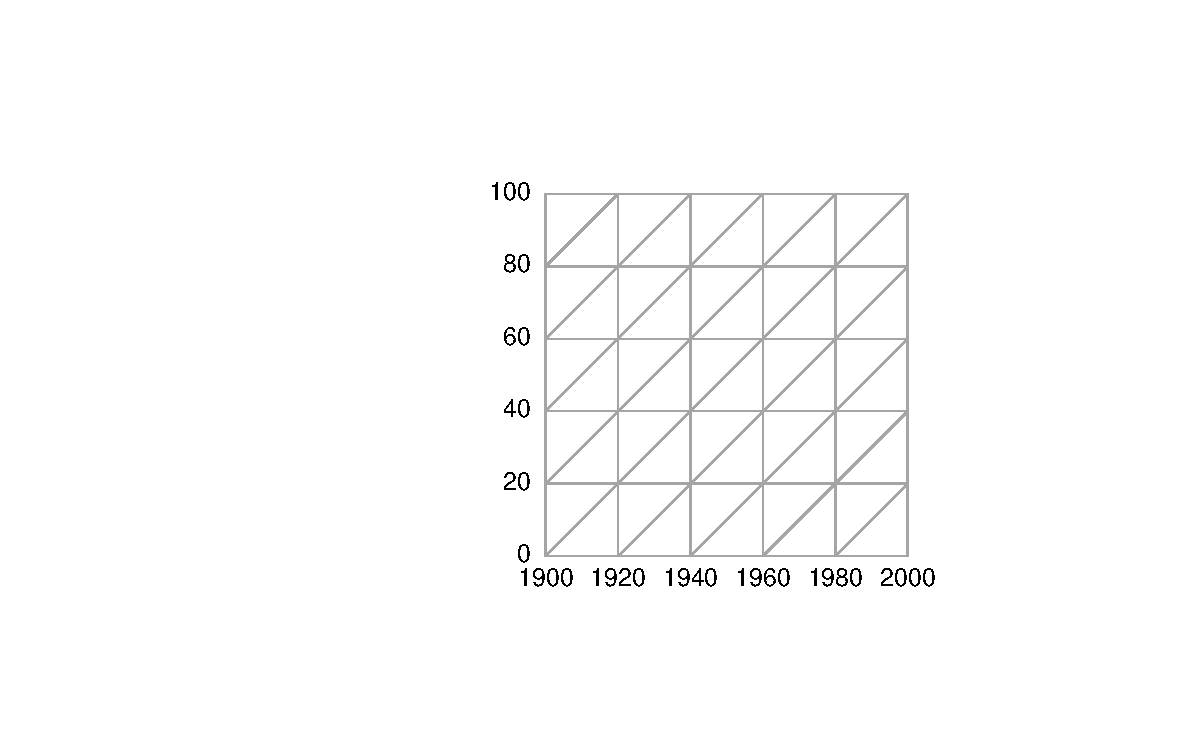
\includegraphics[scale=.7]{Figures/LabPres/APC1.pdf}
    \caption{An APC diagram}
\end{figure} 
\end{frame}

\begin{frame}
\frametitle{An old friend}
\begin{figure}[b]
    \centering
    % figure made in R/LexisStandard.R
    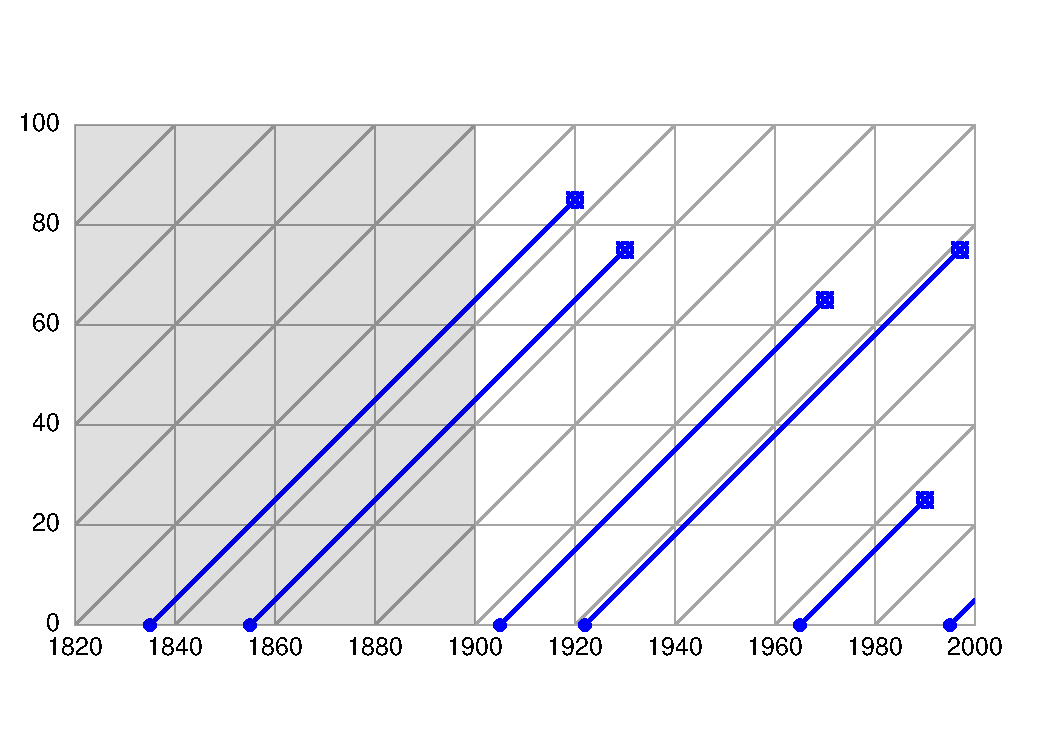
\includegraphics[scale=.7]{Figures/LabPres/APC2.pdf}
    \caption{Lifelines in the APC diagram}
\end{figure} 
\end{frame}

\section{TPD}
\begin{frame}
\frametitle{The inverse relationship}
\begin{figure}[b]
    \centering
    % figure made in R/LexisStandard.R
    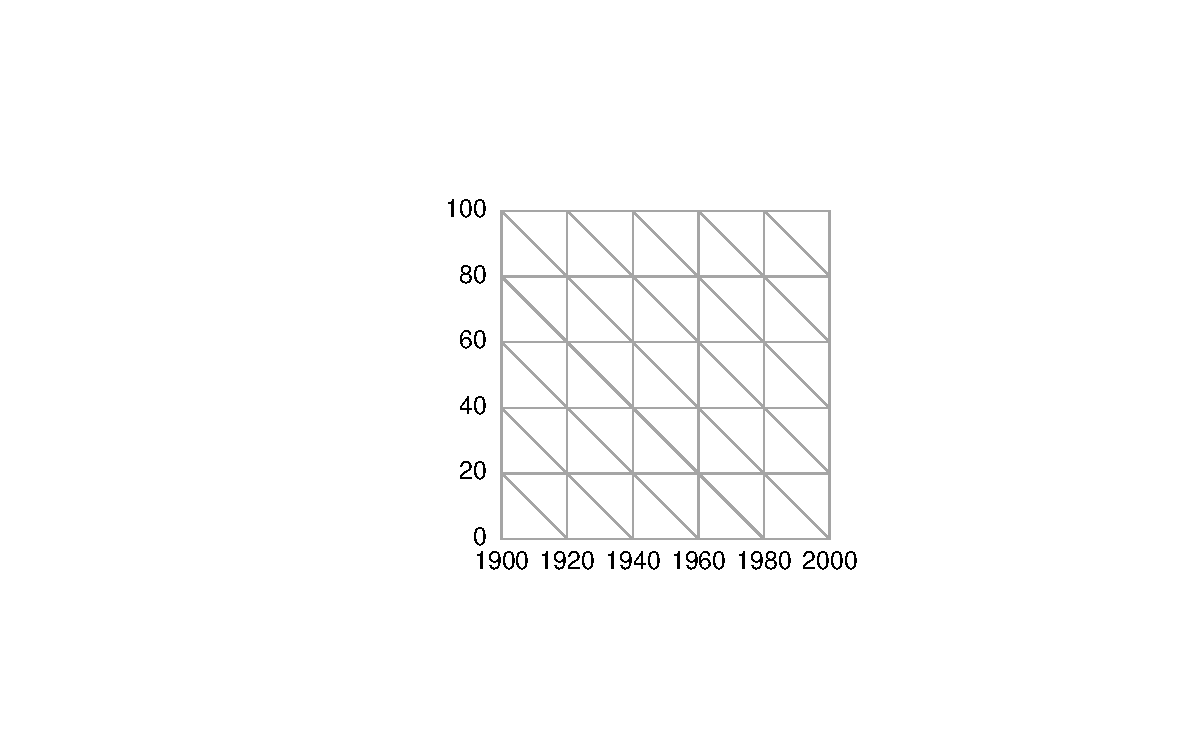
\includegraphics[scale=.7]{Figures/LabPres/TPD1.pdf}
    \caption{A TPD diagram}
\end{figure} 
\end{frame}

\begin{frame}
\frametitle{The inverse relationship}
\begin{figure}[b]
    \centering
    % figure made in R/LexisStandard.R
    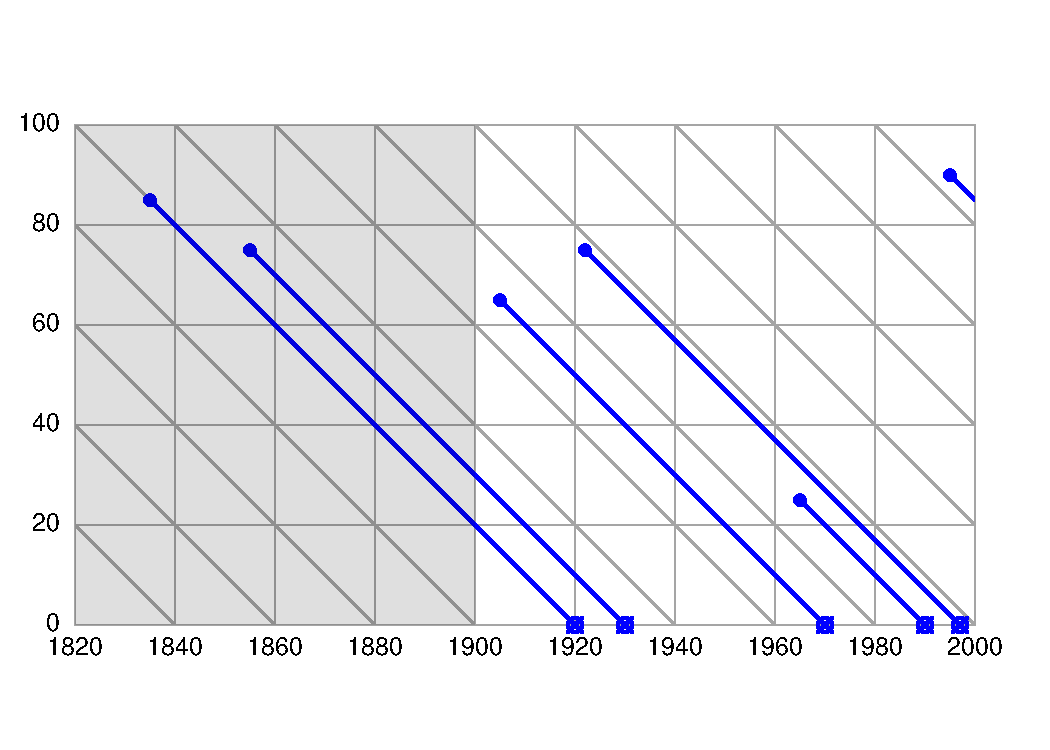
\includegraphics[scale=.7]{Figures/LabPres/TPD2.pdf}
    \caption{Lifelines in the TPD diagram}
\end{figure} 
\end{frame}

\section{TPD}

\end{document}







